\paragraph{Rationale}
These editors are the ones being re-implemented in \gls{cloud}-based \acrshortpl{IDE}.
Understanding their functionality and workings is important, as these editors shape the work of this thesis.
The functionalities provided are assumed highly usable and good, because they are the result of many years of work and experience.
This allows this thesis to skip the work of doing usability testing with regards to feature design, as long as the features are similar enough to the copied ones.

\paragraph{Multiple editors}
When editing \gls{Ecore} models in \gls{Eclipse}, there are different editors to pick from.
Usually, \gls{Ecore} models and model instances are saved as \acrfull{XMI}, which is a standardized serialization format based on XML.
The \gls{Ecore} models have the file extension \texttt{.ecore} while model instances either have \texttt{.xmi} or a custom extension for the model, specified by the modeler (e.g. \texttt{.organization} or \texttt{.courses}).
The GenModel has \texttt{.genmodel} as file extension.
However, \gls{Ecore} models are rarely (if ever) edited as XML.
Instead, the files are loaded and presented in a tree structure editor or diagram editor.
These editors are specialized for \gls{Ecore}, and can understand the model.


The diagram based editors use a notation that is based on \gls{UML} Class Diagrams, with boxes, labels and arrows.
Which editor to use can often be a personal preference.
They are all functionally equivalent, with regards to modeling.
The next subsections will describe the most common tree editors in more detail.

\subsection{Sample Reflective Ecore Model Editor}\label{sec:sample-reflective-editor}

The ``\textit{Sample Reflective Ecore Model Editor}'' is one of the main \gls{Ecore} editors in \gls{Eclipse}.
A screenshot of the editor is shown in \cref{fig:sample-reflective-ecore-model}.
The model instances can be edited in a \textit{reflective} editor (without the user first generating java code and installing an \gls{Eclipse} plugin).
Here, reflective means that the editor uses a metamodel (see \cref{sec:emf-metamodel}) for the model instance, and tries to infer the tree structure from containment relationships.


This editor can open both \gls{Ecore} models and model instances.
A screenshot of a model opened in the editor is shown in \cref{sfig:sample-reflective-ecore-model-screenshot}, and a model instance in \cref{sfig:sample-reflective-ecore-model-instance-screenshot}.


This editor is \gls{open source}%
\footnote{Sample Reflective editor source: \href{https://git.eclipse.org/c/emf/org.eclipse.emf.git/tree/plugins/org.eclipse.emf.ecore.editor}{\nolinkurl{https://git.eclipse.org/c/emf/org.eclipse.emf.git/tree/plugins/org.eclipse.emf.ecore.editor}}.}%
, and the editor is itself originally generated by a genmodel~\cite[p.~10]{rekstadModelingEnvironmentCloud2020}.


This editor internally uses a java class called \texttt{ReflectiveItemProvider}%
\footnote{\texttt{ReflectiveItemProvider} source code: \href{https://git.eclipse.org/c/emf/org.eclipse.emf.git/tree/plugins/org.eclipse.emf.edit/src/org/eclipse/emf/edit/provider/ReflectiveItemProvider.java}{\nolinkurl{https://git.eclipse.org/c/emf/org.eclipse.emf.git/tree/plugins/org.eclipse.emf.edit/src/org/eclipse/emf/edit/provider/ReflectiveItemProvider.java}}}
from the \texttt{org.eclipse.emf.edit} \acrshort{EMF} package, to extract text labels and infer icons for the tree view~\cite[p.~10]{rekstadModelingEnvironmentCloud2020}.


For \gls{Ecore} models (with \texttt{.ecore} file extension, not model instances), it uses an \texttt{EcoreItemProviderAdapterFactory}%
\footnote{\texttt{EcoreItemProviderAdapterFactory} source code: \href{https://git.eclipse.org/c/emf/org.eclipse.emf.git/tree/plugins/org.eclipse.emf.ecore.edit/src/org/eclipse/emf/ecore/provider/EcoreItemProviderAdapterFactory.java}{\nolinkurl{https://git.eclipse.org/c/emf/org.eclipse.emf.git/tree/plugins/org.eclipse.emf.ecore.edit/src/org/eclipse/emf/ecore/provider/EcoreItemProviderAdapterFactory.java}}}
to get labels and icons~\cite{edmerksEcoreEditorJava2021}.


These ``item providers'' are especially interesting, because they could be reused in a new editor.

\begin{figure}
    \centering
    \begin{subfigure}[b]{.45\textwidth}
        \centering
        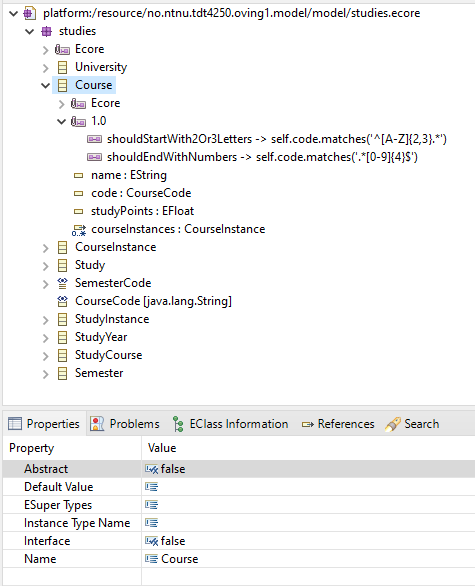
\includegraphics[width=\textwidth]{figures/pre-project/ecore-sample-reflective-ecore-model-editor}
        \caption{A model opened in the editor.}\label{sfig:sample-reflective-ecore-model-screenshot}
    \end{subfigure}
    \hfill
    \begin{subfigure}[b]{.45\textwidth}
        \centering
        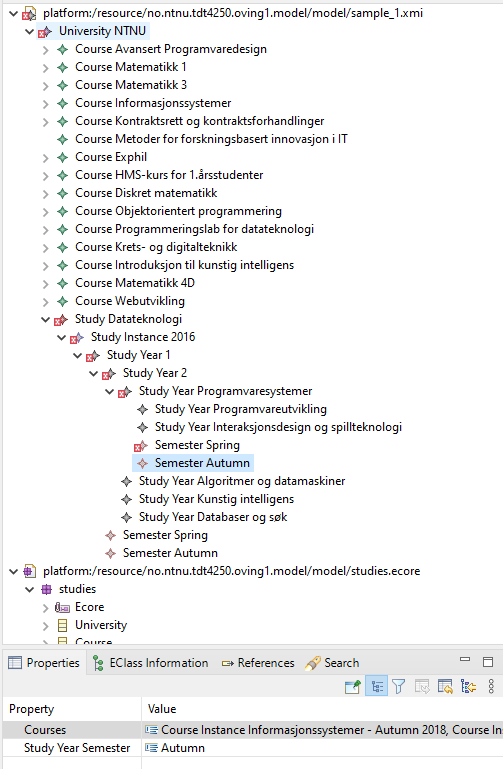
\includegraphics[width=\textwidth]{figures/pre-project/ecore-sample-reflective-ecore-model-editor-instance.png}
        \caption{A \emph{dynamic instance} (\acrshort{XMI} file) opened in the editor.}\label{sfig:sample-reflective-ecore-model-instance-screenshot}
    \end{subfigure}
    \caption{Screenshots of the Sample Reflective Ecore Model Editor in \gls{Eclipse}.}\label{fig:sample-reflective-ecore-model}
\end{figure}


\subsection{EMF Forms Ecore Editor}\label{sec:emfforms-editor}

The \textit{EMF Forms Ecore Editor} is a newer editor than the Sample Reflective editor, and uses EMF Forms\footnote{More info about EMF Forms here: \href{https://www.eclipse.org/ecp/emfforms/index.html}{\nolinkurl{https://www.eclipse.org/ecp/emfforms/index.html}}.} as the technology to provide a user interface~\cite{eclipsesourceEMFFormsEditors2016}.
This editor is \gls{open source}%
\footnote{\textit{EMF Forms} source code: \href{https://git.eclipse.org/c/emfclient/org.eclipse.emf.ecp.core.git/tree/bundles/org.eclipse.emfforms.editor.ecore}{\nolinkurl{https://git.eclipse.org/c/emfclient/org.eclipse.emf.ecp.core.git/tree/bundles/org.eclipse.emfforms.editor.ecore}}.}.
A screenshot of the editor is shown in \cref{fig:emf-forms-ecore-editor}.


This editor is implemented as a generic editor for all \gls{Ecore} model instances, and two subclasses that are specialized for \gls{Ecore} and GenModel~\cite{eclipsesourceEMFFormsEditors2016}.
The generic editor is called \textit{Generic XMI Editor} in \gls{Eclipse}, and the \gls{Ecore} specific editor is called \textit{Ecore Editor}.


The biggest difference compared to the Sample Reflective editor, is how the user interface looks, and that the property sheet is customized based on a \textit{view model file}.
The Sample Reflective editor uses \gls{Eclipse}'s built in property panel.
In the EMF Forms editor, the properties are also grouped into \textit{standard} and \textit{advanced}.

\begin{figure}[htbp]  % order of priority: h here, t top, b bottom, p page
  \centering
  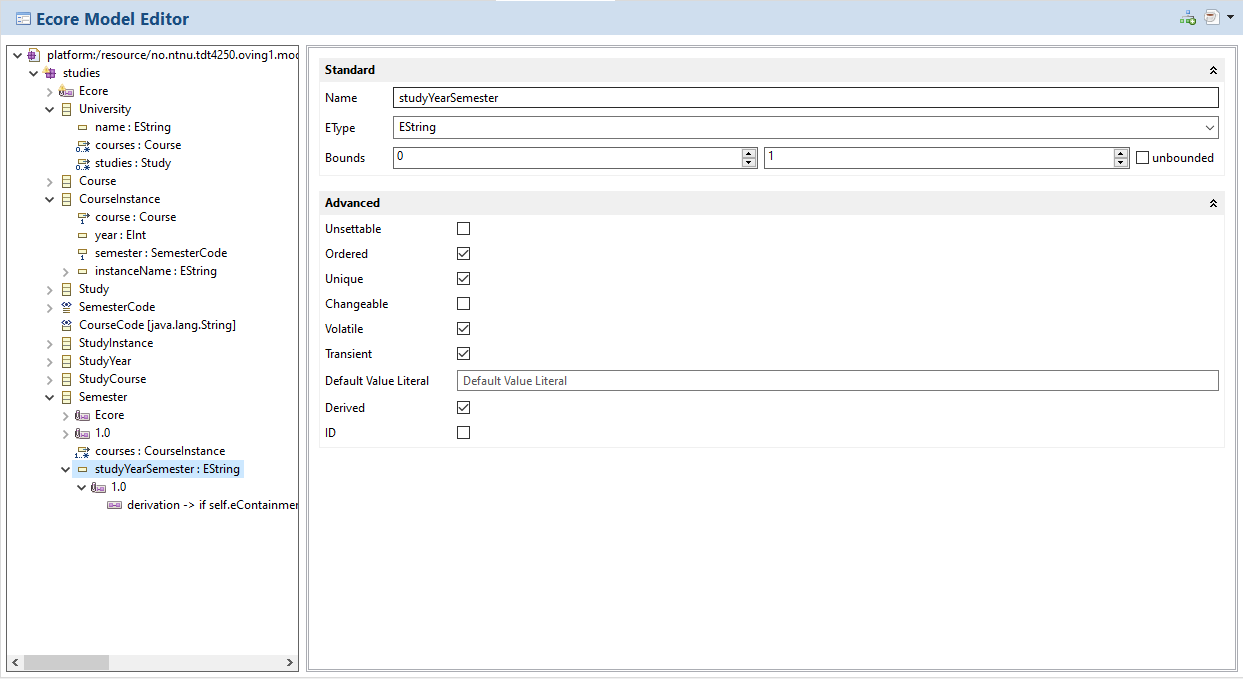
\includegraphics[width=\textwidth]{figures/pre-project/ecore-eclipse-emf-forms-model-editor.png}
  \caption[EMF Forms Ecore Editor]{A screenshot of a model in the EMF Forms based Ecore Editor.}\label{fig:emf-forms-ecore-editor}
\end{figure}

\iffalse{} 
{
%Skip diagrams for now. Tree editors are more important.

  \subsection{Ecore Tools diagrammatical editor}\label{sec:ecore-tools-editor}
  
  The \textit{Ecore Tools} editor presents \gls{Ecore} as class diagrams, similar to \gls{UML} Class Diagrams.
  
  \subsection{EMF.Cloud ecore-glsp diagrammatical editor}\label{sec:ecore-glsp-editor}
  %TODO
  
}
\fi


%* Eclipse EMF offers different Ecore editors. Tree-editor is important for developers, and diagrams are important in runtime and end-users.
